\subsection{Búsqueda con potencias de 2}

\begin{frame}[plain]
  \centering
  \color{theme-brand-color}
  \Huge \textbf{Búsqueda con potencias de 2}
\end{frame}

\begin{frame}{Idea}
  Otra manera de hacer búsqueda binaria es mediante saltos. Si comenzamos en la posición \texttt{pos=0} y en cada iteración avanzamos mientras \texttt{p+jump} no salga del arreglo y \texttt{A[p+jump]} no exceda el valor buscado $x$.\\

  Realizando saltos desde $\frac{N}{2} \rightarrow \frac{N}{4} \rightarrow \cdots \rightarrow 1$, \textit{i.e.}, disminuyendo la velocidad conforme nos acercamos al valor buscado.\\

  Obtenemos una complejidad $\bigO{\log N}$, ya que cada salto puede realizarse a lo más dos veces.
\end{frame}

\begin{frame}{Saltos}
  \begin{figure}[H]
    \centering
    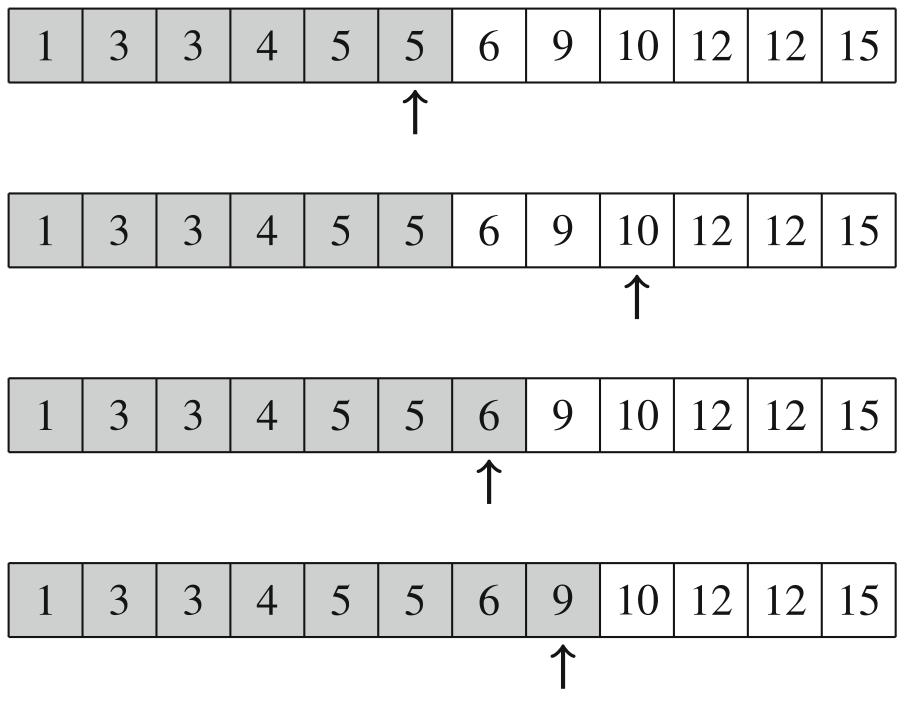
\includegraphics[width=0.65\textwidth]{./assets/idea_powersof2.png}
  \end{figure}
\end{frame}

\begin{frame}[fragile]{Implementación}
  \inputminted[
  fontsize=\large,
  linenos
  ]{cpp}{code/powersof2.cpp}
\end{frame}
